\documentclass[11pt,twocolumn]{article}

\usepackage[brazil]{babel}
\usepackage[utf8]{inputenc}
\usepackage[T1]{fontenc}

\usepackage{graphicx}
\usepackage[caption=false]{subfig}
\usepackage{enumerate}
\usepackage{multirow}
\usepackage{here}


% Definição das variáveis de texto
\title{Exemplo de uso do \LaTeX}
\author{Chauã Queirolo\\Fulano de Tal}
%\date{}

% Local do conteudo do trabalho
\begin{document}
 
\maketitle
\tableofcontents

% Divisão do trabalho
% \part     -> book
% \chapter  -> book, report
% \section  -> todos
% \subsection     -> todos
% \subsubsection  -> todos

\section{Introdução}
\label{sec_introducao}

Nam dictum mauris et diam convallis, sed sagittis dolor blandit. Fusce iaculis, mi eu molestie ullamcorper, lectus nibh scelerisque sem, nec pulvinar massa purus sit amet quam. Integer nec ante et purus lobortis feugiat ac ac velit. Duis pellentesque tincidunt ex, a pulvinar sem pharetra nec. 

Cras egestas velit vel consectetur dapibus. Vivamus in enim sed lacus egestas tempor. Phasellus bibendum sagittis rhoncus. Aliquam semper, turpis vitae vestibulum accumsan, ligula felis cursus quam, vitae suscipit ipsum velit sit amet ipsum. Nunc laoreet erat vel pretium venenatis. Nulla facilisi. Mauris tincidunt nisl vel massa placerat vulputate. Fusce porta est in velit commodo maximus. Sed ac tempor libero.

Nam dictum \textbf{mauris} et diam convallis, sed sagittis dolor blandit. Fusce iaculis, mi eu molestie ullamcorper, lectus nibh scelerisque sem, nec pulvinar massa purus sit amet quam. Integer nec ante et purus lobortis feugiat ac ac velit. Duis pellentesque tincidunt ex, a pulvinar sem pharetra nec. Cras egestas velit vel consectetur dapibus. Vivamus in enim sed lacus egestas tempor. Phasellus bibendum sagittis rhoncus. \textbf{Aliquam semper}, turpis vitae vestibulum accumsan, ligula felis cursus quam, vitae suscipit ipsum velit sit amet ipsum. Nunc laoreet erat vel pretium venenatis. Nulla facilisi. Mauris tincidunt nisl vel massa placerat vulputate. Fusce porta est in velit commodo maximus~(abacate). Sed ac \textit{tempor} libero.

Este trabalho está organizado como segue. A Seção~\ref{sec_fundamentacao} apresenta a fundamentação teórica.

\section{Trabalhos Relacionados}
\label{sec_trabalhos}


\section{Fundamentação Teórica}
\label{sec_fundamentacao}


\subsection{Algoritmo 1}
\label{sec_alg1}

Os Algoritmos Genéticos~(AG) blá blá blá. O aprendizado de máquinas~(\textit{Machine Learning~-~ML}).


\subsection{Algoritmo 2}
\label{sec_alg2}


\section{Tabelas}

De acordo com a Tabela~\ref{tab_exemplo}, os resultados estão abaixo da média.

\begin{table}[h]
  \centering
  \begin{tabular}{l||r|c|c}
    \textbf{Primeira}  & \textbf{Segunda}  & \textbf{Terceira} & \textbf{4} \\
    \hline\hline
    A & B & C & 4\\ \hline
    A & B & C & 4\\ \hline
    A & B & C & 5\\ \hline
  \end{tabular}
 \caption{Exemplo de tabela.}
 \label{tab_exemplo}

\end{table}

\section{Figuras}

De acordo com a Figura~\ref{fig_exemplo}, os resultados estão abaixo da média. 

\begin{figure}[h]
  \centering
  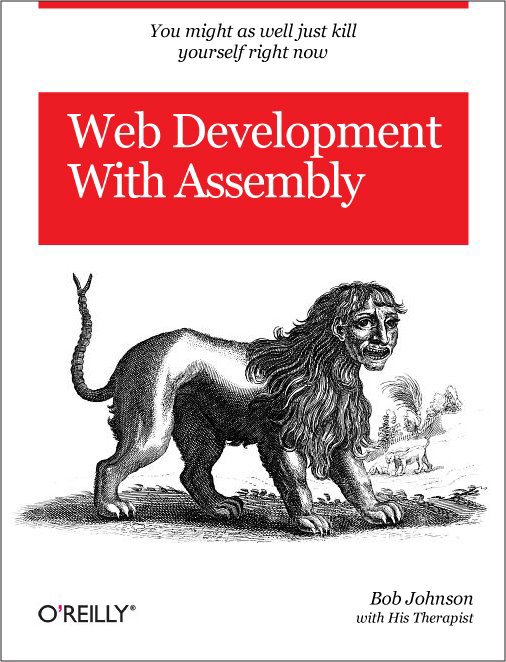
\includegraphics[width=6cm]{exemplo.jpg}
 \caption{Exemplo de figura.}
 \label{fig_exemplo}
\end{figure}

Nam dictum \textbf{mauris} et diam convallis, sed sagittis dolor blandit. Fusce iaculis, mi eu molestie ullamcorper, lectus nibh scelerisque sem, nec pulvinar massa purus sit amet quam. Integer nec ante et purus lobortis feugiat ac ac velit. Duis pellentesque tincidunt ex, a pulvinar sem pharetra nec. Cras egestas velit vel consectetur dapibus. Vivamus in enim sed lacus egestas tempor. Phasellus bibendum sagittis rhoncus. \textbf{Aliquam semper}, turpis vitae vestibulum accumsan, ligula felis cursus quam, vitae suscipit ipsum velit sit amet ipsum. Nunc laoreet erat vel pretium venenatis. Nulla facilisi. Mauris tincidunt nisl vel massa placerat vulputate. Fusce porta est in velit commodo maximus~(abacate). Sed ac \textit{tempor} libero.


\begin{figure}[h]
  \centering
  
  \subfloat[][original]{
    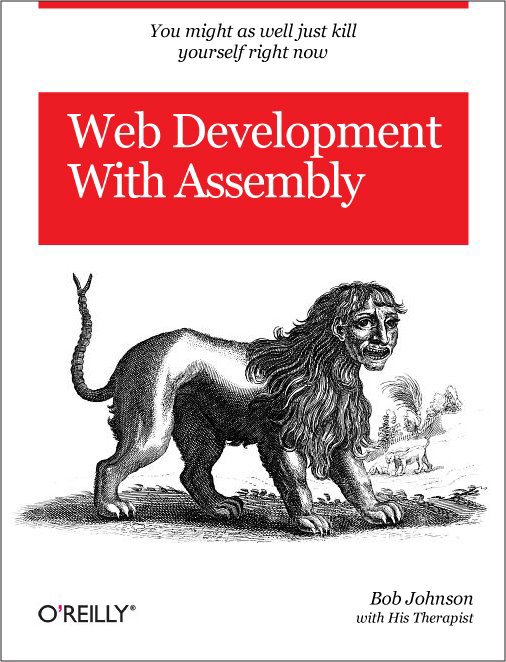
\includegraphics[width=2cm]{exemplo.jpg}
  }  
  \subfloat[][original]{
    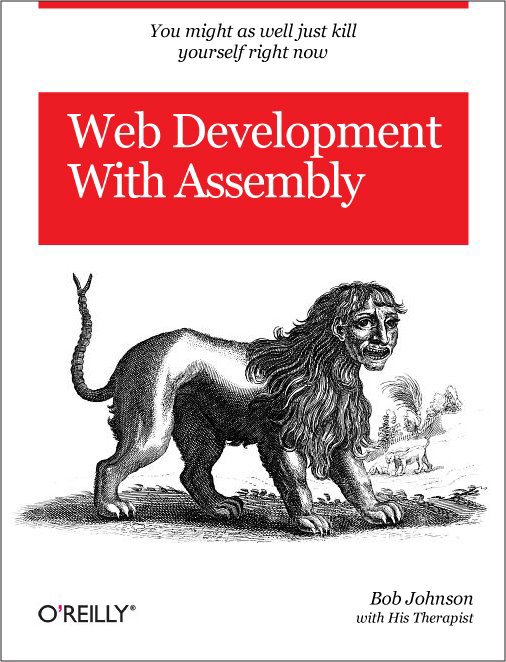
\includegraphics[width=2cm]{exemplo.jpg}
  }
  \subfloat[][original]{
    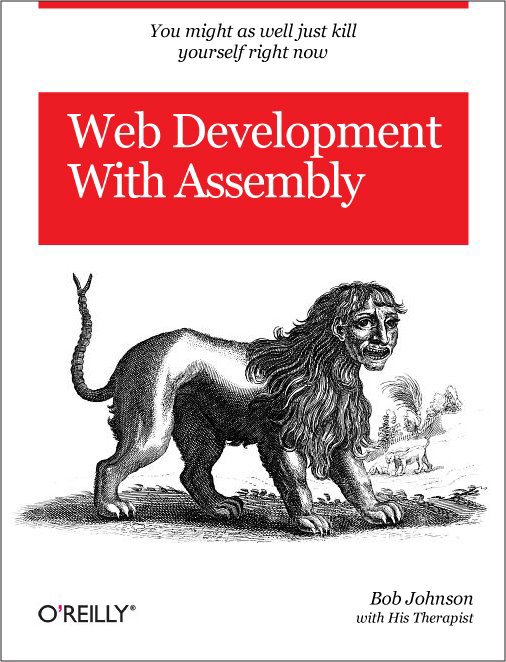
\includegraphics[width=2cm]{exemplo.jpg}
  }
  
  \subfloat[][original]{
    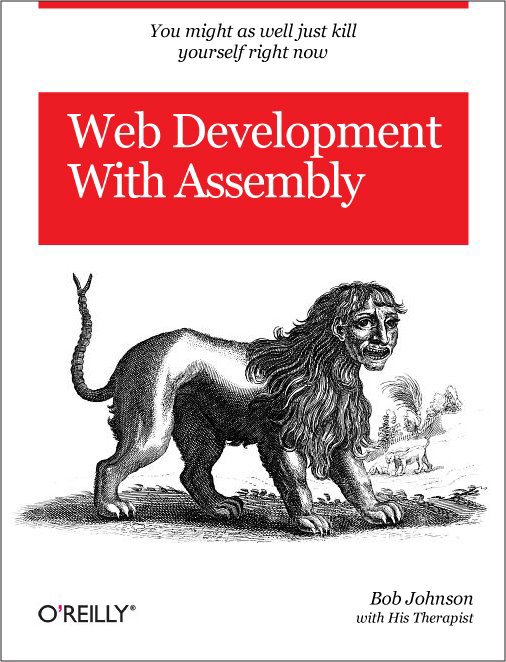
\includegraphics[width=2cm]{exemplo.jpg}
  }
  \subfloat[][original]{
    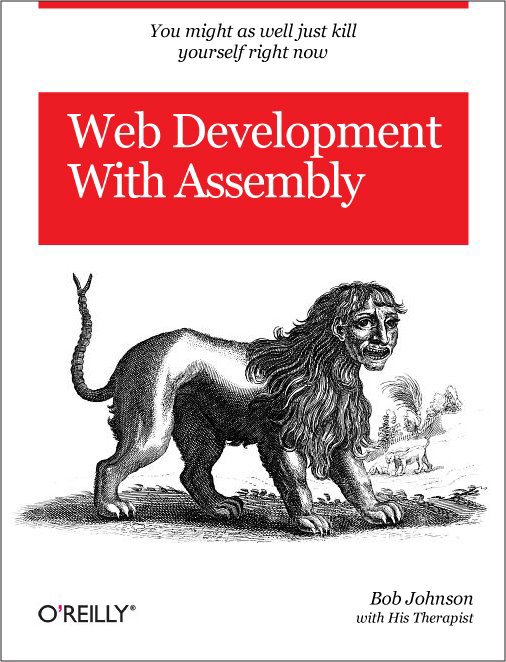
\includegraphics[width=2cm]{exemplo.jpg}
  }  
  
  \caption{Exemplo de subfigura.}
  \label{fig_exemplo2}
\end{figure}


\section{Exemplo de fórmulas}

A variável $x$ é o valor desconhecido, a variável $y$ é a metade de $x$, sendo definida como $y=\frac{1}{2}x$.

A fórmula de Peppers~\cite{berg2006logica} é definida como:

$$
  x = y_1 + y_2 + z^3 + \pi - \delta
$$

A Equação~\ref{eq_peppers} define a média das somas.

\begin{equation}\label{eq_peppers}
A = \frac{\pi r^2}{2} = \frac{1}{2} \pi r^2   
\end{equation} 






\bibliographystyle{acm}
\bibliography{referencias}






  
\end{document}